%%%%%%%%%%%%%%%%%%%%%%%%%%%%%%%%%%%%%%%%%
%
% CMPT 435
% Lab Zero
%
%%%%%%%%%%%%%%%%%%%%%%%%%%%%%%%%%%%%%%%%%

%%%%%%%%%%%%%%%%%%%%%%%%%%%%%%%%%%%%%%%%%
% Short Sectioned Assignment
% LaTeX Template
% Version 1.0 (5/5/12)
%
% This template has been downloaded from: http://www.LaTeXTemplates.com
% Original author: % Frits Wenneker (http://www.howtotex.com)
% License: CC BY-NC-SA 3.0 (http://creativecommons.org/licenses/by-nc-sa/3.0/)
% Modified by Alan G. Labouseur  - alan@labouseur.com
%
%%%%%%%%%%%%%%%%%%%%%%%%%%%%%%%%%%%%%%%%%

%----------------------------------------------------------------------------------------
%	PACKAGES AND OTHER DOCUMENT CONFIGURATIONS
%----------------------------------------------------------------------------------------

\documentclass[letterpaper, 10pt]{article} 

\usepackage[english]{babel} % English language/hyphenation
\usepackage{graphicx}
\usepackage{xcolor}
\graphicspath{ {./images/} }
\usepackage[lined,linesnumbered,commentsnumbered]{algorithm2e}
\usepackage{listings}

% Lstlistings configuration
\definecolor{codegreen}{rgb}{0,0.6,0}
\definecolor{codegray}{rgb}{0.5,0.5,0.5}
\definecolor{codepurple}{rgb}{0.58,0,0.82}
\definecolor{backcolour}{rgb}{0.95,0.95,0.92}

\lstdefinestyle{mystyle}{
    backgroundcolor=\color{backcolour},   
    commentstyle=\color{codegreen},
    keywordstyle=\color{magenta},
    numberstyle=\tiny\color{codegray},
    stringstyle=\color{codepurple},
    basicstyle=\ttfamily\footnotesize,
    breakatwhitespace=false,         
    breaklines=true,                 
    captionpos=b,                    
    keepspaces=true,                 
    numbers=left,                    
    numbersep=5pt,                  
    showspaces=false,                
    showstringspaces=false,
    showtabs=false,                  
    tabsize=2
}

\lstset{style=mystyle}
\lstset{language=Java}

\usepackage{fancyhdr} % Custom headers and footers
\pagestyle{fancyplain} % Makes all pages in the document conform to the custom headers and footers
\usepackage{lastpage}
\usepackage{wasysym}
\usepackage{url}

% Set up for minted package. It had some bugs so I decided to only keep lstlistings.
% \usepackage{minted}
% \makeatletter
% \newlength\minted@belowskip
% \define@key{minted@opt}{belowskip}[\@topsepadd]
% {\setlength{\minted@belowskip}{#1}}

% \def\minted@endparenv{%
%   \addpenalty\@endparpenalty\addvspace\minted@belowskip\@endpetrue}
% \def\FV@EndList{%
%   \FV@ListProcessLastLine
%   \FV@EndListFrame
%   \minted@endparenv
%   \endgroup
%   \@endpetrue}
% \makeatother
% \newminted{java}{linenos=true, belowskip=3cm}

\fancyhead{} % No page header - if you want one, create it in the same way as the footers below
\fancyfoot[L]{} % Empty left footer
\fancyfoot[C]{page \thepage\ of \pageref{LastPage}} % Page numbering for center footer
\fancyfoot[R]{}

\renewcommand{\headrulewidth}{0pt} % Remove header underlines
\renewcommand{\footrulewidth}{0pt} % Remove footer underlines
\setlength{\headheight}{13.6pt} % Customize the height of the header

%----------------------------------------------------------------------------------------
%	TITLE SECTION
%----------------------------------------------------------------------------------------

\newcommand{\horrule}[1]{\rule{\linewidth}{#1}} % Create horizontal rule command with 1 argument of height

\title{	
   \normalfont \normalsize 
   \textsc{CMPT 435 - Fall 2021 - Dr. Labouseur} \\[10pt] % Header stuff.
   \horrule{0.5pt} \\[0.25cm] 	% Top horizontal rule
   \huge Assignment One -- Finding Palindromes \\     	    % Assignment title
   \horrule{0.5pt} \\[0.25cm] 	% Bottom horizontal rule
}

\author{Augusto Gonzalez-Bonorino \\ \normalsize augusto.gonzalezbonorino1@marist.edu}

\date{\normalsize\today} 	% Today's date.

\begin{document}

\maketitle % Print the title

%----------------------------------------------------------------------------------------
%   CONTENT SECTION
%----------------------------------------------------------------------------------------

% - -- -  - -- -  - -- -  -

\section{Description of the program}

The program described in this document can be, conceptually, divided into two parts: Implementation of Stack, Queue and a singly linked list; utilizing the aforementioned data structures to find palindromes in a given text document.

It consists of four classes: StackGonzalezBonorino, QueueGonzalezBonorino, MainGonzalezBonorino and NodeGonzalezBonorino. The characteristics and methods of each class will be described in more detail throughout this documentation. \\

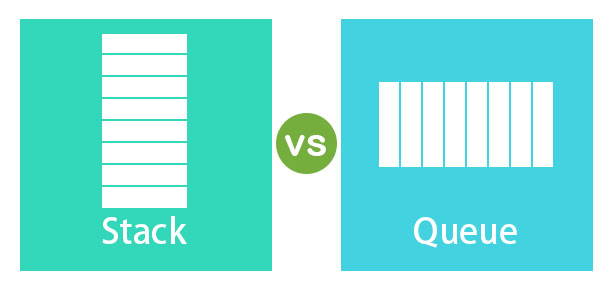
\includegraphics[scale=0.5]{images/Stack.jpg}

\pagebreak
\section{Stack class}

In this section I will describe in detail how I have designed my Stack data structure. In the words of Lewis Carroll "Let's begin at the beginning". 
\\
The following extract of code corresponds to the initialization of the necessary instances and default constructor:

\begin{lstlisting}
/**
 * 
 * @author Augusto Gonzalez Bonorino
 *
 * This is the class definition for StackGonzalezBonorino
 */
public class StackGonzalezBonorino 
{
	/**
	 * Instance variable for the top of the stack
	 */
	private NodeGonzalezBonorino myTop;
	
	/**
	 * Default constructor for StackGonzalezBonorino
	 */
	public StackGonzalezBonorino() {
		
		myTop = null;
	} // default constructor

\end{lstlisting}

Next, I defined a function to check if the Stack is empty which comes in handy to avoid hitting a null value while looping through the elements of the Stack.

\begin{lstlisting}
 /**
 * Method to check if Stack is empty
 * @return boolean true if empty false otherwise
 */
public boolean isEmpty() {
	
	if (myTop == null)
		return true;
	else
		return false;
} // check if empty
\end{lstlisting}

Lastly, the two most important methods in the Stack are \textit{push()} and \textit{pop()} which are used to add and delete elements from the Stack, respectively.

The method \textit{push()} assigns the element it receives (in this case a character) to the variable \textit{myTop}, which represent the top of the Stack. Then, it assigns the element previously located at the top to a variable I called \textit{oldTop}, thereby adding a new element to the Stack.

\begin{lstlisting}
/**
 * Method to add elements to the Stack
 * @param element
 */
public void push(char element) {
	
	NodeGonzalezBonorino oldTop = myTop;
	myTop = new NodeGonzalezBonorino();
	myTop.setData(element);
	myTop.setNext(oldTop);
	
} //push
\end{lstlisting}

The method \textit{pop()} extracts and returns the element located at the top of our Stack. Note that before considering deleting an element we must check that the Stack is not empty, otherwise we would try to access a \textbf{null} value and that would raise a \textit{\textbf{NullPointerException}} and nobody wants that \smiley{}. Then, if the stack is not empty it assigns the element at \textit{myTop} to the local variable \textit{ans}, updates the top and returns \textit{ans}.

\begin{lstlisting}
/**
 * Method to delete and element from the Stack
 * @return element extracted
 */
public char pop() {
	
	char ans = ' ';
	
	if (!(isEmpty())) 
	{	
		ans = myTop.getData();
		myTop = myTop.getNext();
	} //if
	else {
		System.out.println("Stack is empty"); } //else
	
	return ans; } // pop
\end{lstlisting}

\section{Queue class}
The queue is a data structure that follows a particular order, referred to as First In First Out (FIFO), in which  the operations are performed.
\\
As always, the first thing to do is declare and instantiate the necessary variables for the class. For a Queue we need a variable that refers to the head of the queue and one that refers to the tail, I have called these \textit{myHead} and \textit{myTail} respectively.
\begin{lstlisting}
/**
 * 
 * @author Augusto Gonzalez Bonorino <br><br>
 *
 * This is the class definition for QueueGonzalezBonorino
 */
public class QueueGonzalezBonorino {
	
	/**
	 * Instance variable for the queue's tail
	 */
	private NodeGonzalezBonorino myTail;

	/**
	 * Instance variable for the queue's head
	 */
	private NodeGonzalezBonorino myHead;
	
	/**
	 * Default constructor for QueueGonzalezBonorino
	 */
	public QueueGonzalezBonorino() {
		
		myTail = null;
	} // constructor
\end{lstlisting}

Next, just like for our Stack, we need a method to make sure the Queue is not empty.

\begin{lstlisting}
/**
	 * Method to check if Queue is empty
	 * @return boolean true if empty false otherwise
	 */
	public boolean isEmpty() {
		
		if (myHead == null)
			return true;
		else
			return false;
	} // check if empty
\end{lstlisting}

Now, we need a way to add and delete elements. This is achieved by the methods \textit{enqueue()} and \textit{dequeue()}.

In the enqueue method I first declare a new \textit{NodeGonzalezBonorino} variable to hold the element previously at the tail of the queue. Next, \textit{myTail} is updated by creating a new \textit{NodeGonzalezBonorino}, setting its data to the element the user inputted and setting the next node to \textbf{null}. Then, we have to set the head of the queue if the Queue is empty (meaning that if the element being added is, currently, the only one on the Queue both \textit{myHead} and \textit{myTail} are equal) or update the Node to which \textit{oldTail} is pointing at. 
\begin{lstlisting}
/**
	 * Method to add elements to the Queue
	 * @param element
	 */
	public void enqueue(char element) {
		
		NodeGonzalezBonorino oldTail = myTail;
		myTail = new NodeGonzalezBonorino();
		myTail.setData(element);
		myTail.setNext(null);
		
		if (isEmpty())
			myHead = myTail;
		else
			oldTail.setNext(myTail);
	} //enqueue
\end{lstlisting}

The dequeue method is implemented in the following fashion: A local variable to hold the character to be extracted is initialized which I creatively called \textit{ans}, we make sure the Queue is not empty (otherwise Java would raise a \textit{\textbf{NullPointerException}}), assign the data extracted to \textit{ans} and update the value of \textit{myHead} by getting the value of the node it's pointing to. It is worth mentioning that if we are extracting the last element of the queue the data structure will be empty afterwards. Thus, we need to make sure that if this is the case we set \textit{myTail} to null. This is implemented in lines 14-15. 
\begin{lstlisting}
/**
	 * Method to delete and element from the Queue
	 * @return element extracted
	 */
	public char dequeue() {
		
		char ans = ' ';
		
		if (!isEmpty()) {
			
			ans = myHead.getData();
			myHead = myHead.getNext();
			
			if (isEmpty())
				myTail = null;
			
		} //if
		
		else
			System.out.println("Queue is empty");
		
		return ans;
		
	} //dequeue
	
} // QueueGonzalezBonorino
\end{lstlisting}


\section{Node class (Singly linked list)}

Linked list is a special data structure that allows us to go beyond regular arrays by linking elements to pointers instead of storing them in a contiguous location. Thus, the linked list is not bounded by a predetermined length like regular arrays. Also, it is "singly" linked because it only points to the element the comes next, unlike "doubly" linked lists which can move forwards and backwards. I leverage this data structure to implement both the Stack and the Queue. 

Our Node class contains two variables on is used to hold the data, which I conveniently called \textit{myData}, while the second is an instance of itself used to point (link) to the next node in the list, which I also conveniently called \textit{myNext}. In addition, it contains the common default constructor and a not-so-common semi-constructor that gives us the flexibility to assign \textit{myData} a new value.

\begin{lstlisting}
/**
 * 
 * @author Augusto Gonzalez Bonorino
 * This is the class definition for NodeGonzalezBonorino
 * 
 */
public class NodeGonzalezBonorino {
	/**
	 * Instance variable to hold the data
	 */
	private char myData;
	
	/**
	 * Instance variable for the data of the next node
	 */
	private NodeGonzalezBonorino myNext;
	
	/**
	 * Default constructor for NodeGonzalezBonorino
	 */
	public NodeGonzalezBonorino() {
		
		myData = ' ';
		myNext = null;
		
	} // Default Constructor
	
	/**
	 * Semi-constructor for NodeGonzalezBonorino
	 * @param newData value to assign the data to myData
	 */
	public NodeGonzalezBonorino(char newData){
		
		myData = newData;
		myNext = null;
		
	} // Semi-constructor
\end{lstlisting}

Besides the unusual semi-constructor there is nothing really interesting to explore in detail in the remaining code. The following lines of code correspond to the getters and setter of the class.

\begin{lstlisting}
/**
	 * Method to get myData
	 * @return myData
	 */
	public char getData() {
		
		return myData;
	} // getData
	
	/**
	 * Method to get the value of the next node
	 * @return myNext
	 */
	public NodeGonzalezBonorino getNext() {
		
		return myNext;
	} //getNext
	
	/**
	 * Method to set the value of myData
	 * @param newData
	 */
	public void setData(char newData) {
		
		myData = newData;
	} //setData
	
	/**
	 * Method to set the value of myNext
	 * @param newNext
	 */
	public void setNext(NodeGonzalezBonorino newNext) {
		
		myNext = newNext;
	} // setNext
	
} // Node
\end{lstlisting}

\section{Main class}

Great, but how do I actually find cool palindromes? Well, all the fun stuff takes place in the MainGonzalezBonorino class. First, like with any class, I import the packages needed to process user input and read external files (util and io). Then, I instantiate all the variables I will use throughout the program and read the file with the following code:

\begin{lstlisting}
import java.util.*;
import java.io.*;
/**
 * 
 * @author Augusto Gonzalez Bonorino <br>
 * 
 * assignment1GonzalezBonorino <br>
 * Due Date and Time: 09/24/21 before 9:00 a.m. <br><br>
 *
 * Purpose: Develop program that leverages a singly linked list, stacks and queues to find palindromes. <br><br>
 *			
 * Input: A text file containing the words or sentences to check for palindromes.
 * 		  
 * Output: The program prints out those words or sentences that were indeed palindromes.<br><br>
 *		   
 *
 * Certification of Authenticity: <br>
 * 
 * I certify that this assignment is entirely my own work. <br>
 */
public class MainGonzalezBonorino {
	
	static Scanner keyboard = new Scanner(System.in);
	
	public static void main(String[] args) {
		
		File theMagicFile = null;
		
		String fileName = "magicitems.txt";
		String tempString = null;
		
		String [] myMagicList = new String[666];
		int numItems = 0;
		
		String ans = "\nSome suggestions: \n"
				+ "\n* Check that the name of the file was typed correctly"
				+ "\n* Make sure that you are not missing any information in your item description in the file"
				+ "\n* Make sure you are not entering more or less items than specified";
		
		try
		{
			System.out.print("Enter the name of the file: ");
			fileName = keyboard.next();
			
			theMagicFile = new File(fileName);
			
			Scanner input = new Scanner(theMagicFile);
			
			while(input.hasNextLine()) {
				
				tempString = input.nextLine();
				myMagicList[numItems] = tempString;
				
				numItems++;
				
			} //while 
			
			input.close();
			
		} //try
		
		catch(IndexOutOfBoundsException ex)
	    {
			System.out.println("Oops, something went wrong!");
			System.out.println("It seems that the program has reached an index out of bounds.");
\end{lstlisting}

Note the usage of \textit{try} and \textit{catch} when reading the file. There are more exceptions being taken into account but I excluded them from this snippet of code to avoid crowding the documentation with irrelevant code. Basically, after the user inputs the name of the file, the program reads each line \textit{while} the file still has a line to read and appends it to an array. The usage of the while loop provides greater flexibility and cleaner code, which is why I prefer it over the for loop.

Once the file has been completely read, and the array fully populated, we must loop through every element in the array and push/enqueue it to a Stack and a Queue. For this, I use three loops. The \textit{outer for loop} goes through every element in the array, the \textit{inner for loop} adds every character in that respective element to our Stack and Queue, and the \textit{while} loop which then extracts and compares each character. In order to find our \textit{coolWord} it is necessary to "normalize" every String in the array. I achieve this by eliminating all white spaces and capitalizing every character in the String (note that this is done in the outer loop, every time a new element is read).  

\begin{lstlisting}

		for (int i = 0; i < myMagicList.length; i++) {
			
			StackGonzalezBonorino stack = new StackGonzalezBonorino();
			QueueGonzalezBonorino queue = new QueueGonzalezBonorino();
			String coolWord = myMagicList[i].replaceAll(" ", "").toUpperCase();
			
			
			for (int j = 0; j < coolWord.length(); j++) {
				
				char c = coolWord.charAt(j);
				
				stack.push(c);
				queue.enqueue(c);
				
				
			} //inner for loop
			
			boolean isPalindrome = true;
			
			while ( !stack.isEmpty() && isPalindrome) {
				
				char elemS = stack.pop();
				char elemQ = queue.dequeue();
				if (Character.compare(elemS, elemQ) != 0)
					isPalindrome = false;
				
			} //while
				
			if(isPalindrome)
				System.out.println(myMagicList[i]);
			
		} //Outer for loop
		
		
	} // main

} // MainGonzalezBonorino
\end{lstlisting}

Inside the outer for loop is really where the magic happens. So, to ensure the reader comprehends it I will expand on its design a little further. Here are the inner loops extracted from the previous listing of code:
\begin{lstlisting}
for (int j = 0; j < coolWord.length(); j++) {
				
				char c = coolWord.charAt(j);
				
				stack.push(c);
				queue.enqueue(c);
				
				
			} //inner for loop
			
			boolean isPalindrome = true;
			
			while ( !stack.isEmpty() && isPalindrome) {
				
				char elemS = stack.pop();
				char elemQ = queue.dequeue();
				if (Character.compare(elemS, elemQ) != 0)
					isPalindrome = false;
				
			} //while
				
			if(isPalindrome)
				System.out.println(myMagicList[i]);
\end{lstlisting}
First, I take each character on our \textit{coolWord} one by one and add it to both the Stack and the Queue. Then, the \textit{while} loop pops/dequeues an element from both the Stack and the Queue, check if they are the same, and proceeds in the same fashion until the characters are different. If the \textit{while} loop goes over the entire word, then \textit{isPalindrome} remains true and the program prints our \textit{coolWord}. Do this for every word in the text file and Voila! We have found all the palindromes in the given document.

\section{Final thoughts}

Documentation is about explaining how the program works and how it was designed. But, it does not have to be just that, here are a few funny palindromes to sweeten this report:
\\
\\ % source: https://www.grammarly.com/blog/16-surprisingly-funny-palindromes/
First we have a great bargain:\\
A nut for a jar of tuna.\\
But there's always someone unwilling to give up a nut, so he hired a hitman with the following pitch line:\\
Murder for a jar of red rum.
\\
\\
And a funny meme to conclude this document:\\
\begin{center}
    
\includegraphics[scale=0.3]{images/palindromeMeme.jpg}
\end{center}



\end{document}